\chapter{Torus Trick}\label{c13}

This\pageoriginale lecture is devoted to giving Quinn's proof from
\cite{84} of Lemma \ref{c12:lem12.4}. The key to his argument is
constructing a geometric group version of Kirby's torus trick
\cite{66}. To do this, Quinn makes crucial use of the Bass-Heller-Swan
Theorem \cite{5} which states that $Wh \Gamma =0$ when $\Gamma$ is a
free abelian group.

Identify the $n$-torus $T^n$ with the quotient group
$\mathbb{R}^n/(3\mathbb{Z})^n$. Then, $\mathbb{D}^n \subset T^n$. See
Figure 12.
\begin{figure}[H]
  \centering{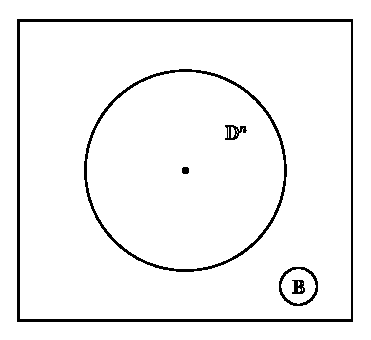
\includegraphics{vol86-figures/fig12.eps}\\
  Figure 12}
\end{figure}

Let $\mathbb{B}$ be a second small closed $n$-dimensional round ball
which is disjoint from $\mathbb{D}^n$ in $T^n$. And let 
$$
j: T^n - \Int \left(\frac{1}{2}\mathbb{B} \right) \to \frac{2}{3} \mathbb{D}^n
$$
be a smooth immersion such that $j\mid_{\frac{1}{2}
  \mathbb{D}^n}=id$. Let $0\mathbb{B}$ denote the center of
$\mathbb{B}$. More generally, let
\begin{align*}
  r \mathbb{B} & = \{ x \in \mathbb{B}\mid d (x, 0 \mathbb{B}) \leq
  r\} ~\text{and}~\\
  r \mathbb{D}^n & = \{ x \in \mathbb{R}^n \mid ~ \mid x\mid \leq r \}
\end{align*}
where $0 \leq r \leq 1$. Such an immersion exists because of the
Smale-Hirsch immersion theorem and the fact that $T^n-0\mathbb{B}$ is
parallelizable. An explicit such immersion, when $n=2$, can
constructed by considering Figure 13.
\begin{figure}[H]
  \centering{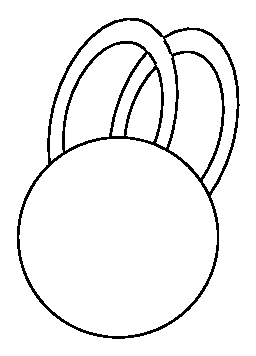
\includegraphics{vol86-figures/fig13.eps}\\
  Figure 13}
\end{figure}

Given\pageoriginale a geometric group $G$ with basis $x_1, \ldots , x_m$ on
$\mathbb{D}^n$, define a geometric group $j^* G$ on $T^n - \Int \left(
\frac{1}{2} \mathbb{B}\right)$ with basis
$\displaystyle{\bigcup_{i=1}^m \left\{j^{-1} (x_i) \right\}}$. The
order of the basis elements in $j^* G$ is ambiguously determined; but
this is unimportant. Fix a positive real number $\gamma$ satisfying
the following conditin:
\begin{equation*}
  \text{If} ~ d(x, y)\leq 2 \gamma ~\text{and}~ j(x) = j(y),
  ~\text{then}~x=y. \tag{0}
\end{equation*}

Such numbers exist since $j$ is an immersion with compact domain. We
also choose $\gamma$ to be smaller than the number $\epsilon$ given in
the hypotheses of Lemma \ref{c12:lem12.4}. The following assertion is
also a consequence of the fact that $j$ is an immersion. These exists
a number $\delta > 0$ such that, for each $a \in T^n- \left(\gamma +
\frac{1}{2} \right)\mathbb{B}$ and each $b \in \mathbb{D}^n$ with $d(j
(a), b)\leq \delta$, the equation $j(x) =b$ has a unique solution $x
\in T^n- \frac{1}{2} \mathbb{B}$ subject to the constraint $d(x,
a)\leq \gamma$. This property allows us to associate to any
$\delta$-homomorphism $f: G \to G$ a $\gamma$-homomorphism $\ob{f} :
j^* G \to j^* G$ such that $\ob{j} \circ \ob{f}$ and $f \circ \ob{j}$
are equal when restricted to $T^n - \left(\gamma + \frac{1}{2}
\right)\mathbb{B}$. Here, $\ob{j}: j^* G \to G$ is the canonical
homomorphism induced by the natural basis correspondence. Furthermore,
$\ob{f}$ restricted to $T^n- \left(\gamma + \frac{1}{2}
\right)\mathbb{B}$ is uniquely determined. (Note the similarity
between this construction and the second construction of $\hat{f}$
given in \ref{c11:sec11.3}.)

This\pageoriginale uniqueness property shows that if $f$ is a
$\delta$-automorphism over $\frac{2}{3} \mathbb{D}^n$, then $\ob{f}$
is a $\gamma$-automorphism over $T^n- (2 \gamma +
\frac{1}{2})\mathbb{B}$. We assume from now on that $f$ is the
$\delta$-automorphism given in the statement of the Lemma
\ref{c12:lem12.4}. Let $\mathcal{G}_0 = j^* G\mid_{T^n - \frac{2}{3}
  \mathbb{B}}$ and $\mathcal{G}_1= j^* G\mid_{\frac{2}{3}
  \mathbb{B}}$. Hence, $j^* G = \mathcal{G}_0 \oplus
\mathcal{G}_1$. Using that $\ob{f}$ is a $\gamma$-automorphism over
$T^n - (2 \gamma + \frac{1}{2})\mathbb{B}$, it is seen that $\ob{f}
(\mathcal{G}_0)$ is also a direct summand of $j^* G$. Stated more
precisely
$$
\mathcal{G} = \ob{f} (\mathcal{G}_0) \oplus \mathcal{G}_3
$$ 
where $\mathcal{G}_3$ is a subgroup of $j^*
G\mid_{\frac{3}{4}\mathbb{B}}$. But the Fundamental Theorem of
Finitely Generated Abelian Groups implies that $\mathcal{G}_1 \simeq
\mathcal{G}_3$. Using these facts, we can construct an automorphism
$\ob{f}_1: j^* G \to j^* G$ such that 
\begin{gather*}
  \ob{f}_1 \mid_{T^n- \frac{2}{3} \mathbb{B}}= \ob{F} ~\text{and}\\
  \ob{f} (\mathcal{G}_1) \subset j^* G\mid_{\frac{3}{4}\mathbb{B}}.
\end{gather*}

It is easy to construct a self-diffeomorphism $g: T^n \to T^n$ with
the following properties:
\begin{enumerate}
\item $g\mid_{T^n -\mathbb{B}}= id$.
\item $\diam  g \left(\frac{3}{4} \mathbb{B} \right)\leq \gamma$.
\item $|dg (v)| \leq 4 \mid v\mid$ for each vector $v$ tangent to $T^n$. 
\end{enumerate}

A new geometric group $G_1$ on $T^n$ is constructed by applying $g$ to
the basis elements of $j^* G$. This process also yields a new
automorphism $f_1: G_1 \to G_1$ such that 
\begin{enumerate}
\item $f_1$ is a $4 \gamma$-automorphism, and 
\item $f_1 \mid_{\frac{1}{2}\mathbb{D}}=f$.
\end{enumerate}

Assuming $4 \gamma \leq 1$, we can form the square matrix $\hat{f}_1$
with entries from $\mathbb{Z}(\pi_1 T^n)$. If we use its second
construction from \ref{c11:sec11.3} to do this, then $\hat{f}_1$ can
be regarded as an automorphism of the ``geometric group'' $p^* G_1$
over $\mathbb{R}^n$, where $p: \mathbb{R}^n \to T^n = \mathbb{R}^n/(3
\mathbb{Z}^n)$ is\pageoriginale the canonical projection. Considered
this way, $p^* G_1$ is a free but not finitely generated
$\mathbb{Z}$-module. It is however a free and finitely generated
$\mathbb{Z} (\pi_1 T^n)$-module.

Quinn now uses the Fundamental Theorem of Algebraic $K$-theory, due to
Bass-Heller-Swan \cite{5}; this results states that
$$
Wh (\pi_1 T^n)=0.
$$

It allows him to factor $\hat{f}$ as a certain product
\begin{equation*}
  E_k e_{k-1} \cdots E_1 E_0 \tag{1}\label{c13:eq1}
\end{equation*}
after stablizing $\hat{f}$ outside the orbit of $\frac{1}{2}
\mathbb{D}^n$ under the action of $\pi_1 (T^n)$. The matrix $E_0$, in
this factorization, is \textit{strongly diagonal}; i.e., only its
first (diagonal) entry is possibly not equal 1 and that entry is
either $\alpha$ or $-\alpha$ for some $\alpha \in \pi_1 (T^n)$. The
matrices $E_i$ (for $i>0$) \textit{are strongly elementary}; i.e., the
non-zero off diagonal entry of $E_i$ is $a_i \alpha_i$ where $a_i
\in \mathbb{Z}$ and $\alpha_i \in \pi_1 (T^n)$. Let $G_2$ be a
geometric group over $T^n- \frac{1}{2} \mathbb{D}^n$ such that $p^*
(G_1 \oplus G_2)$ is the stabilization in the factorization
\eqref{c13:eq1}.

Now fix a very large positive real number $s$. How large will be
presently evident. We proceed next to modify each of the automorphisms
$$
E_i : p^* (G_1 \oplus G_2) \to p^* (G_1 \oplus G_2)
$$
where $i = 0, 1, \ldots , k$. We change $E_i$ to a new automorphism
$\mathcal{E}_i$ satisfying the following properties:
\begin{enumerate}
\item $\mathcal{E}_i \mid_{s\mathbb{D}^n}= E_i \mid_{s \mathbb{D}^n}$;
  \item $\mathcal{E}_i \mid_{\mathbb{R}^n}= id$;
    \item $\diam  \mathcal{E}_i= \diam  \mathcal{E}_i^{-1} \leq \diam  E_i$.
\end{enumerate}

The $\mathcal{E}_i$ are automorphisms of $\hat{\mathcal{G}}= p^* (G_1
\oplus G_2) \oplus~ G_3$ where $G_3$ is a (finitely generated)
geometric group on $\mathbb{R}^n- s\mathbb{D}^n$. Also each
$\mathcal{E}_i$, where $i \geq 1$, is blocked relative to the
subgroups $p^* (G_1 \oplus G_2)$ and $G_3$ so that
$\mathcal{E}_i\mid_{G_3}=id$. Note that each $E_i (i \geq
1)$ is blocked via\pageoriginale a partition of the basis of $p^* (G_1
\oplus G_2)$ into subsets containing either 1 or 2 elements. And the
matrix representing $E_i$ on the 2 element partitions is 
$$
\begin{pmatrix}
  1 & a_i\\
  0 & 1
\end{pmatrix}
$$

Also each 2 element member of the partiton relative to $E_i$ has the
same diameter. Then $\mathcal{E}_i$ is determined by changing the
matrix
$$
\begin{pmatrix}
  1 & a_i\\
  0 & 1
\end{pmatrix}~\text{to}~
\begin{pmatrix}
  1 & 0\\
  0 & 1
\end{pmatrix}
$$
on each 2 element member of this partition which meets $\mathbb{R}^n -
2 s \mathbb{D}^n$.

Note that $E_0$ is blocked relative to a partition $\mathcal{P}$
consisting of singletons and infinite sets $S_t$ where each $S_t$ lies
on a straight line $L_t$ in $\mathbb{R}^n$. The set $S_t$ divides
$L_t$ into intervals of constant length $l$, independent of the index
$t$. Furthermore, $E_0$ maps each point in $S_t$ one unit $l$ in the
same direction. For each $L_t$ that intersects $s\mathbb{D}^n$,
draw a smooth curve in $2s\mathbb{D}^n-s\mathbb{D}^{n}$ 
connecting the first exit
point on $L_t$ to the first entrance point. (Note this is impossible
to do when $n=1$.) See Figure 14.
\begin{figure}[H]
  \centering{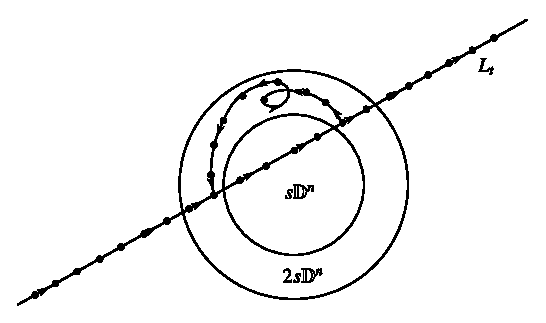
\includegraphics{vol86-figures/fig14.eps}\\
  \qquad Figure 14}
\end{figure}

Introduce new basis elements along these curves so that the distance
between successive elements is $\leq l$. These new points are the
basis for $G_3$. Define $\mathcal{E}_0$ to circulate around
the\pageoriginale new cycles just constructed as indicated in Figure
14, and to be  the identify off these cycles.

It is clear that the automorphisms $\mathcal{E}_i$ thus constructed
satisfy conditions 1, 2, and 3 posited above. Furthermore, when $s$ is
sufficiently large, each $\mathcal{E}_i$ is blocked relative to the
decomposition
$$
\hat{\mathcal{G}} \hat{\mathcal{G}} \mid_{3 s\mathbb{D}^n} \oplus
\hat{\mathcal{G}}\mid_{\mathbb{R}^n - 3 s\mathbb{D}^n} 
$$
and is the identity map on the second factor.

It is easy to construct a diffeomorphism $h: 3 s\mathbb{D}^n \to
\mathbb{D}^n$ having the following three properties:
\begin{enumerate}
\item $h\mid_{\frac{2}{3} \mathbb{D}^n} = id$;
  \item $|dh (v)| \leq \mid v \mid$ for each vector $v$ tangent to $3
    s\mathbb{D}^n$;
    \item $|dh (v)| \leq \frac{1}{s} \mid v\mid$ for each vector $v$
      tangent to $3 s\mathbb{D}^n - s\mathbb{D}^n$.
\end{enumerate}

A new geometric group $\hat{\mathcal{G}_1}$ on $\mathbb{D}^n$ is
constructed by applying $h$ to the basis elements of
$\hat{\mathcal{G}}\mid_{3 s \mathbb{D}^n}$. And conjugating
$\mathcal{E}_k \mathcal{E}_{k-1}\cdots \mathcal{E}_1 \mathcal{E}_0
\mid_{3 s \mathbb{D}^n}$ with the geometric automorphism induced by
$h$ yields an automorphism $\mathcal{E} : \hat{\mathcal{G}_1} \to
  \hat{\mathcal{G}_1}$. Let the geometric group $H$ posited in Lemma
  \ref{c12:lem12.4} be $\hat{\mathcal{G}}_1 \mid_{\mathbb{D}^n -
    \frac{1}{2} \mathbb{D}^n}$, and notice that 
$$
G \oplus H = G\mid_{\mathbb{D}^n - \frac{1}{2} \mathbb{D}^n} \oplus\;
\hat{\mathcal{G}}_1.
$$

Set $\ob{f} =id \oplus \mathcal{E}$ relative to this
decomposition. Then $\ob{f} \mid_{\frac{2}{5}\mathbb{D}^n}
=f\mid_{\frac{2}{5} \mathbb{D}^n}$ and $\ob{f}$ is a $4
\gamma$-automorphism provided $s$ is chosen to be sufficiently
large. If we pick $4 \gamma \leq \epsilon$ and $s$ sufficiently large,
then this proves Lemma \ref{c12:lem12.4}.

